\documentclass[14pt, a4paper, ukrainian]{extreport}

\usepackage[14pt]{extsizes}
\usepackage{cmap}
\usepackage[utf8]{inputenc}
\usepackage[T2A]{fontenc}
\usepackage[english, ukrainian]{babel}
\usepackage{slashbox}
\usepackage{caption}
\DeclareCaptionLabelFormat{gostfigure}{Рисунок #2}
\DeclareCaptionLabelFormat{gosttable}{Таблиця #2}
\DeclareCaptionLabelSeparator{gost}{~---~}
\captionsetup{labelsep=gost}
\captionsetup*[figure]{labelformat=gostfigure}
\captionsetup*[table]{labelformat=gosttable}
\captionsetup*[figure]{labelformat=gostfigure, justification=centering}  % выравнивание по центру



\usepackage{titlesec}

\titleformat{\chapter}[block]
{\filcenter}
{\thechapter}
{1em}
{\MakeUppercase}
{}

\titlespacing*{\chapter}{0pt}{-40pt}{*4} 

\titleformat{\section}
{\filright}
{\thesection}
{1ex}{}

\titleformat{\subsection}
{\filright}
{\thesubsection}
{1ex}{}

%Clickable contents list
\usepackage{hyperref}
\hypersetup{
	pdftitle={Розрахунково-графічна робота},
	pdfauthor={Олександр Вергелюк},
	linkbordercolor= 1 1 1
}


\title{Розрахунково-графічна робота}
\author{Олександр Вергелюк}
\date{\today}


\usepackage[left=3.00cm, right=1.50cm, top=2.00cm, bottom=2.00cm]{geometry}

%Робота з математикою 
\usepackage{graphicx}
\usepackage{amsmath, amsfonts, amssymb, mathtools} %AMS
\usepackage{icomma} %Розумна кома
\usepackage{indentfirst}
\parindent 1.25cm
\usepackage[usenames,dvipsnames]{color}
\usepackage{makecell}
\usepackage{multirow}
\usepackage{ulem}
\usepackage{float}

%Шрифти
\usepackage{euscript}
\usepackage{mathrsfs}
\linespread{1.3} % полуторный интервал

\begin{document}
	\begin{titlepage}
		\centering
		\vspace{1cm}
		{ МІНІСТЕРСТВО ОСВІТИ І НАУКИ УКРАЇНИ\\
			НАВЧАЛЬНО-НАУКОВИЙ КОМПЛЕКС\\
			``ІНСТИТУТ ПРИКЛАДНОГО СИСТЕМНОГО АНАЛІЗУ``\\
			НАЦІОНАЛЬНОГО ТЕХНІЧНОГО УНІВЕРСИТЕТУ УКРАЇНИ\\
			``КИЇВСЬКИЙ ПОЛІТЕХНІЧНИЙ ІНСТИТУТ ІМЕНІ ІГОРЯ СІКОРСЬКОГО``\\
			КАФЕДРА МАТЕМАТИЧНИХ МЕТОДІВ  СИСТЕМНОГО АНАЛІЗУ\\\par}
		\vspace{5cm}
		\MakeUppercase {\textsc{\textbf{{розрахунково-графічна робота №2}}}}\\
		{з математичної статистики} \\
		\vfill
		\newlength{\ML}
		\settowidth{\ML}{\hspace{3.4cm}}
		\hfill
		\begin{minipage}{0.35\textwidth}
			Виконав студент 2 курсу групи КА-06\\
			Вергелюк Олександр\\ Андрійович
			
			Перевірив: \\
			Ільєнко Андрій\\ Борисович
		\end{minipage}
		\vfill
		\begin{center}
			Київ --- 2022
		\end{center}
	\end{titlepage}
	\setcounter{page}{2}
	\renewcommand\contentsname{Зміст}
	\tableofcontents
	\chapter*{Вступ}
	\addcontentsline{toc}{chapter}{Вступ}
	У файлі svyato.txt знайти свій набір із 100 чисел. Вони імітують вибірку, отриману із генеральної сукупності.
	
	\begin{center}
		Дана вибірка \linebreak
		
		\begin{tabular} {c c c c c c c c c c}
			-3.47 & 0.06 & -1.11 & -3.77 & 1.13 & 2.23 & -3.51 & -3.2 & -0.64 & -1.61 \\ 
			0.06 & -1.11 & -3.77 & 1.13 & 2.23 & -3.51 & -3.2 & -0.64 & -1.61 & -2.44 \\ 
			-1.11 & -3.77 & 1.13 & 2.23 & -3.51 & -3.2 & -0.64 & -1.61 & -2.44 & -5.44 \\ 
			-3.77 & 1.13 & 2.23 & -3.51 & -3.2 & -0.64 & -1.61 & -2.44 & -5.44 & -0.6 \\ 
			1.13 & 2.23 & -3.51 & -3.2 & -0.64 & -1.61 & -2.44 & -5.44 & -0.6 & 1.94 \\ 
			2.23 & -3.51 & -3.2 & -0.64 & -1.61 & -2.44 & -5.44 & -0.6 & 1.94 & -2.46 \\ 
			-3.51 & -3.2 & -0.64 & -1.61 & -2.44 & -5.44 & -0.6 & 1.94 & -2.46 & -1.12 \\ 
			-3.2 & -0.64 & -1.61 & -2.44 & -5.44 & -0.6 & 1.94 & -2.46 & -1.12 & -3.85 \\ 
			-0.64 & -1.61 & -2.44 & -5.44 & -0.6 & 1.94 & -2.46 & -1.12 & -3.85 & -1.0 \\ 
			-1.61 & -2.44 & -5.44 & -0.6 & 1.94 & -2.46 & -1.12 & -3.85 & -1.0 & -1.18 
		\end{tabular}
	\end{center}
	
	\begin{center}
		Відсортована вибірка \linebreak
		
		\begin{tabular} {c c c c c c c c c c}
		 -6.78 & -6.57 & -5.48 & -5.44 & -5.21 & -5.08 & -4.49 & -4.37 & -4.36 & -4.11 \\
		 -3.98 & -3.97 & -3.92 & -3.85 & -3.77 & -3.6 & -3.51 & -3.49 & -3.47 & -3.44 \\
		 -3.43 & -3.34 & -3.22 & -3.2 & -3.18 & -3.09 & -3.05 & -2.99 & -2.96 & -2.84 \\
		 -2.75 & -2.73 & -2.48 & -2.46 & -2.45 & -2.44 & -2.34 & -2.1 & -1.99 & -1.96 \\
		 -1.95 & -1.94 & -1.91 & -1.91 & -1.91 & -1.78 & -1.74 & -1.64 & -1.63 & -1.61 \\
		 -1.55 & -1.5 & -1.48 & -1.39 & -1.34 & -1.29 & -1.18 & -1.15 & -1.12 & -1.11 \\
		 -1.08 & -1.02 & -1.0 & -0.91 & -0.85 & -0.76 & -0.71 & -0.64 & -0.6 & -0.49 \\
		 -0.48 & -0.46 & -0.04 & -0.03 & 0.06 & 0.11 & 0.12 & 0.16 & 0.21 & 0.31 \\
		 0.32 & 0.4 & 0.44 & 0.87 & 0.99 & 1.05 & 1.13 & 1.16 & 1.18 & 1.24 \\
		 1.28 & 1.32 & 1.86 & 1.94 & 2.1 & 2.23 & 2.26 & 2.48 & 3.28 & 3.52
	\end{tabular}
	\end{center}

	Постановка задачі:
	
	\begin{enumerate}
		\item Проведіть первинний аналіз вибірки. Ци включає статистичний ряд (для неперервних розподілів --- інтервальний), емпіричну функцію розподілу (для неперервних розподілів --- інтервальну), її графік, полігон частот (для дискретних розподілів), гістограму (для неперервних розподілів), box-and-whisker plot.
		
		\item Знайдість вибіркове середнє, вибіркову дисперсію, виправлену вибіркову дисперсію, вибіркову медіану, вибіркову моду, вибіркові коефіцієнти асиметрії та ексцесу.
		
		\item \underline{Обґрунтуйте} та висуньте (нову) гіпотезу про розподіл генеральної сукупності.
		
		\item Методом моментів та методом максимальної вірогідності знайдіть оцінки параметрів розподілу. В деяких випадках це може бути не дуже просто (як, наприклад, для параметру \textit{N} біноміальної генеральної сукупності). Це чудовий спосіб проявити креативність та/або вміння користуватися Google.
		
		\item Для кожного параметру кращу у цих двох оцінок перевірте на \break
		(асимптотичну) незміщеність, консистентність та ефективність. Тут також має сенс зауваження до попереднього пункту. У випадку \break нездоланних труднощів --- а це відноситься \underline{виключно} до перевірки ефективності \textit{a} та \textit{b} в U(\textit{a, b}), \textit{a} в Exp(\textit{y, a}) та \textit{N} в Bin(\textit{N, p}) --- відповідну перевірку можно пропустити.
		
		\item Побудуйте довірчі інтервали надійністю 0.95 для параметрів розподілу. (The above notes still apply!)		
		
		\item Нарешті перевірте висунуту гіпотезу про розподіл генеральної сукупності за допомогою критерію $\chi^2$. Якщо гіпотеза суперечить вибірковим даним, перейдіть до п.3.
		
		\item Проявiть всi свої лiтературнi здiбностi та напишiть висновки.
		
	\end{enumerate}

	Інструменти, що я використовував під час роботи над цією РГР:
	\begin{itemize}
		\item Jupyter notebook
	\end{itemize}
	
	\chapter{Первинний аналіз вибірки}
	
	З загального виду вибірки видно, що її переважну більшість становлять раціональні числа, серед яких лише одне значення повторюється. Отже, можна висунути припущення, що надана вибірка з неперервного розподілу генеральної сукупності. Подальший аналі вибірки буде наподитися для випадку неперервного розподілу.
	
	Побудуємо інтервальний ряд для вибірки. Для цього за формулою Стерджеса визначимо кількість інтервалів.
	$$N_{intervals} = 1 + 3.322 * \lg n \approx 8$$
	Тепер знайдемо розмах вибірки, щоб обрати довжини інтервалів.
	$$R = x_{(n)} - x_{(1)} = 3.52 - (-6.78) = 10.3$$
	
	Для зручності в подальшому оберемо однакові довжини для всіх інтервалів причому такі, щоб точки, які визначають межі інтервалів мали лише один знак після коми.
	$$h = \frac{R}{N_{intervals}} = \frac{10.3}{8} \approx 1.3$$
	Тепер можемо побудувати статистичний ряд, табл. \ref{tab:stats}.
	\begin{table}[H]
		\caption{\label{tab:stats} Інтервальний статистичний ряд}
		\begin{center}
			\begin{tabular}{| l | l | l | l | l | l |}
				\hline
				$\Delta_k$ 	 & $x_k^*$ & $n$ & $n^*$ & $\nu$ & $\nu^*$ \\
				\hline
				[-6.8 ;  -5.5) & -6.15 &   2 &     2 &  0.02 &    0.02 \\
				\hline
				[-5.5 ;  -4.2) & -4.85 &   7 &     9 &  0.07 &    0.09 \\
				\hline
				[-4.2 ;  -2.9) & -3.55 &  20 &    29 &   0.2 &    0.29 \\
				\hline
				[-2.9 ;  -1.6) & -2.25 &  21 &    50 &  0.21 &     0.5 \\
				\hline
				[-1.6 ;  -0.3) & -0.95 &  22 &    72 &  0.22 &    0.72 \\
				\hline
				[-0.3 ;   1.0) &  0.35 &  13 &    85 &  0.13 &    0.85 \\
				\hline
				[ 1.0 ;   2.3) &  1.65 &  12 &    97 &  0.12 &    0.97 \\
				\hline
				[ 2.3 ;   3.6] &  2.95 &   3 &   100 &  0.03 &     1 \\
				\hline
			\end{tabular}
		\end{center}
	\end{table}
	
	Тепер за статистичним рядом можна побудувати емпіричну інтервальну функцію розподілу.
	$$ F_n^*(x) =
	\begin{cases}
		0 & x \le -6.8\\
		0.02 & -6.8 < x \le -5.5\\
		0.09 & -5.5 < x \le -4.2\\
		0.29 & -4.2 < x \le -2.9\\
		0.5 & -2.9 < x \le -1.6\\
		0.72 & -1.6 < x \le -0.3\\
		0.85 & -0.3 < x \le 1\\
		0.97 & 1 < x \le 2.3\\
		1 & 2.3 < x \le 3.5\\
	\end{cases} 
	$$
	
	Графік цієї функції наведено на рис. \ref{im:distribution_func}.
	\begin{figure}[H]
		\centering
		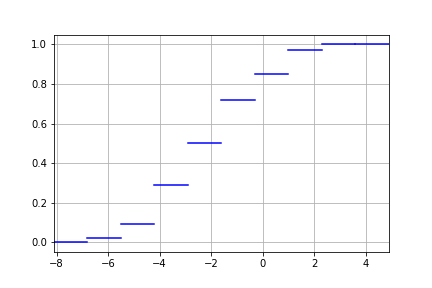
\includegraphics[width=0.8\textwidth]{./Image/CDF.png}
		\caption{Графік емпіричної інтервальної функції розподілу}
		\label{im:distribution_func}
	\end{figure}

	Гістограма для даної вибірки наведена на рис. \ref{im:hist}
	\begin{figure}[H]
		\centering
		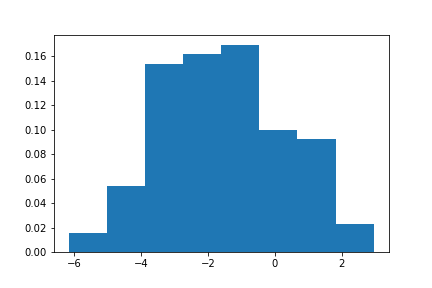
\includegraphics[width=0.8\textwidth]{./Image/Histogram.png}
		\caption{Гістограма даної вибірки}
		\label{im:hist}
	\end{figure}
	
	Тепер побудуємо діаграму box-and-whisker (ящик з вусами) для даної вибірки (рис. \ref{im:box_and_whisker}).
		\begin{figure}[H]
		\centering
		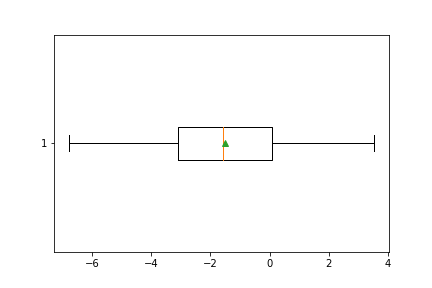
\includegraphics[width=0.8\textwidth]{./Image/Box_and_whisker.png}
		\caption{Box-and-whisker}
		\label{im:box_and_whisker}
	\end{figure}	
	
	\chapter{Описові стастики}
	Тепер знайдемо описові статистики вибірки: вибіркове середнє, вибіркову дисперсію, виправлену вибіркову десперсію, вибіркову медіану, мибіркову моду, вибіркові коефіцієнти асиметрії та ексцесу.
	
	Знайдемо вибіркове середнє:
	$$ \overline{x} = \frac{1}{n}\sum_{i=1}^{n}x_i = -1.5207$$
	
	Тепер обчислимо вибіркову дисперсію
	$$ \mathbb{D}\xi^{**} = \frac{1}{n}\sum_{i=1}^{n}(x_i - \overline{x})^2 = 4.5888$$
	
	Знайдемо виправлену вибіркову дисперсію
	$$ \mathbb{D}\xi^{***} = \frac{1}{n-1}\sum_{i=1}^{n}(x_i - \overline{x})^2 = 4.6352$$
	
	Оскільки в нашій вибірці n = 100, то медіана вибірки:
	$$ M_e^* = \frac{x_{(50)} + x_{(51)}}{2} = \frac{-1.61 - 1.55}{2} = -1.58$$
	
	Оскільки наша вибірка з неперервного розподілу генеральної сукупності, то вибіркова мода визначається за формулою:
	$$ M_o^* = y_{mo-1} + h \frac{n_i - n_{i-1}}{(n_i - n_{i-1}) + (n_i - n_{i+1})} = $$
	$$ = -1.6 + 1.3\frac{22 - 21}{(22 - 21) + (22 - 13)} = - 1.47$$

	Обчислимо вибірковий коефіцієнт асиметрії:
	$$ A_s = \frac{\overline{M_3}}{s_0^3} = \frac{\sum_{i=1}^{n}(x_i - \overline{x})^3}{ns_0^3} = 0.0318$$
	
	Знайдемо вибірковий коефіцієнт ексцесу:
	$$ E_k = \frac{\overline{M_4}}{s_0^4} - 3= \frac{\sum_{i=1}^{n}(x_i - \overline{x})^4}{ns_0^4} - 3 = -0.3145$$
		
	\chapter{Гіпотеза про розподіл генеральної сукупності}
	
	Оскільки з самого початку було прийнято припущення, що генеральна сукупність має неперервний розподіл, то логічно визначати можливий розподіл із неперервних. За умовою, це можуть бути 3 варіанти:
	\begin{itemize}
		\item гаусівський;
		\item рівномірний;
		\item експоненціальний із зсувом.
	\end{itemize}
	
	\chapter{Оцінка параметрів розподілу}
	\chapter{Перевірка параметрів на незміщеність, консистентність та ефективність}
	\chapter{Довірчі інтервали для параметрів розподілу}
	\chapter{Перевірка висунотої гіпотези за критерієм $\chi^2$}
	\chapter*{Висновки}
	\addcontentsline{toc}{chapter}{Висновки}	
	
	
\end{document}